\documentclass[
  ngerman
  ,12pt
  ,pdftex
]{article}

\usepackage{graphicx}
\usepackage{amsmath}
\usepackage{amssymb}
\usepackage{listings}
\usepackage[ngerman]{babel}
\usepackage[utf8]{inputenc}
\usepackage[T1]{fontenc}
\usepackage{alltt}
\usepackage{pdfpages}
\usepackage{setspace}
\usepackage[a4paper,margin=2cm]{geometry}
\usepackage{footnote}
\usepackage{tikz}
\makesavenoteenv{tabular}
\makesavenoteenv{table}
\setstretch{1.3}



\begin{document}

\tableofcontents
\section{Deskriptive Statistik (Wahrscheinlichkeitstheorie)}

Gegeben sei die Stichprobe $x=(x_1,..,x_n)$ vom Umfang $n$ mit Werten in $\mathbb{R}$.
\[\overline{x}:= \frac{1}{n}*\sum_{i = 1}^{n}=\frac{x_1+...+x_n}{n}     \]

heißt Stichproben-Mittel,

\[{s_x}^2:=\frac{1}{n-1}\sum_{i=1}^{n}(x_i-\overline{x})^2   =\frac{(x_1-\overline{x})^2+...+(x_n-\overline{x})^2}{n-1}\]

Stichproben-Varianz, wobei $n\geq 2$

\[s_x := +\sqrt{{s_x}^2} \]

Stichproben-Standaedabweichung und

\[v_x := \frac{s_x}{x} \]

für $x_1,...,x_n >0 $ heißt Stichproben-Variantionskoeffizient.\\

Der Stichproben-Median (Zentralwert) von $x$

\[\tilde{x} :=\begin{cases}x_{(\frac{n+1}{2})}\textrm{    ,falls $n$ ungerade}\\
    \frac{1}{2}*(x_{(\frac{n}{2})}+x_{(\frac{n}{2}+1)})\textrm{ ,falls n gerade}\end{cases}\]

Stichproben -$\alpha$-Quantil\\

Sei $\alpha \in (0,1)$ und $k:=[n*\alpha]$. Dann heißt

\[\tilde{x}_\alpha  :=\begin{cases}x_{(k+1)}\textrm{,falls $n*\alpha \notin \mathbb{N} $}\\
    \frac{1}{2}*(x_{(k)}+x_{(k+1)})\textrm{,sonst}\end{cases}\]


$\alpha$-getrimmte Stichproben-Mittel(kommt nicht dran)\\

Sei $\alpha \in [0,0.5]$ und $k:=[n*\alpha ]$. Dann heißt

\[\tilde{x}_\alpha := \frac{1}{n-2*k}*(x_{(k+1)}+...+x_{(n-k)}) \]

das $\alpha $-getrimmte (gestutzte) Stichproben-Mittel.


\subsection{Wahrscheinlichkeitsräume}

auch Stochastisches Modell Zufallsexperiment\\
ist ein Tripel($\Omega ,\mathcal{E}, \mathbb{P}$)
\begin{itemize}
    \item [i] Grundraum $\Omega\neq \varnothing  $
    \item [ii] Ereignisraum $\varepsilon $
    \item [iii] Wahrscheinlichkeitsmaß $\mathbb{P}$
\end{itemize}
$\mathbb{P} :\varepsilon \longleftarrow [0,1]$ weißt jedem Ereignis eine Wahrscheinlichkeit zu.\\

Wie berechent man das Wahrscheinlichkeitsmaß?\\
\renewcommand{\labelenumi}{\alph{enumi})}
\begin{enumerate}
    \item $\mathbb{P}(\emptyset) = 0$
    \item $\mathbb{P} (\sum_{j = 1}^{n} A_j)=\sum_{j = 1}^{n}\mathbb{P} (A_j) $ ,falls $A_1,...,A_n$ paarweise disjunkt (endliche Additivität)
    \item $\mathbb{P} (A^c)= 1-\mathbb{P} (A)$, $\forall A:A\in \mathcal{A} \longleftarrow A^c\in \mathcal{A} $
    \item $A\subset B \longleftarrow \mathbb{P}(A)\leq \mathbb{P} (B)$(Monotonie)
    \item $\mathbb{P} (A\cup B)=\mathbb{P} (A)+\mathbb{P} (B)-\mathbb{P} (A\cap B)$
\end{enumerate}
c) Wegen $\Omega = A+A^c$ und b) gilt $1 = \mathbb{P} (\Omega)=\mathbb{P} (A)+\mathbb{P} (A^c)$.

genauers wird in den Späteren Vorlesung erläutert.\\

\section{Kombinatorik}
Erscheint ein Laplace-Modell in einer Situation angemessen, so ist die Wahrscheinlichkeit eines Ereignisses $A$

\[P(A)=\frac{\textrm{Anzal der für $A$ \dq günstigen \dq Fälle}}{\textrm{Anzal aller mölicen Fälle}} \]

Die Lere vom systematischen Abzlen endlicher \dq strukturierter \dq Mengen heißt Kombinatorik.

\subsection{Multiplikationsregel (Produktregel)}

\[m_1\cdot m_2 \cdot ... \cdot m_k\]

Beispiele: Wie viele Möglichkeiten ggibt es jeweils?\\

\begin{itemize}
    \item Auf der Speisekarte stehen 3 Vorspeisen, 10 Hauptgerichte und 2 Desserts. Wie viele 3-gängige Menüs kann man zusammenstellen? $\Longrightarrow 3\cdot 10\cdot 2 = 60$
    \item Ein roter und ein blauer Würfel werden geworfen.$\Longrightarrow 6\cdot 6=36$
    \item Bei einem Neuwagen gibt es 8 aufpriespflichtige Zusatzoptionen, die in beliebiger Kombination zu- oder abbestellt werden können.$\Longrightarrow 2\cdot 2\cdot ...\cdot 2 = 2^8=256$
\end{itemize}

Wenn es Experminente sind in denen zurückgelegt wird kann die \texttt{Produktregel nicht angewendet} werden, da Werte nicht beliebig kombinierbar sind.


\subsection{Summenregel}

Wenn es mehrere Gruppen mit $m_1$ bzw. $...m_n$ verschiedenen Werte gibt, die sich gegenseitig ausschließen, dann gibt es insgesamt $m_1+...+m_n$ mögliche Werte.\\

\texttt{Beispiel}\\
Auf der Speisekarte sind als Hauptspeise 10 Fleischgerichte, 4 Fischgerichte und 2 vegetarische Gerichte zur Auswahl. Zusätzlich gibt es 3 Vorspeisen und 5 Desserts zur Auswahl. Wie viele 3 gängige Menüs kann man zusammenstellen?

\[3\cdot (10+4+2)\cdot 5=240\]

\subsection{Permutation u. Kombinationen}

Tabelle wird nachgereicht solbald internet\\

Hier ist:

\begin{align}
    \binom{m}{l}&:=\frac{m!}{l!\cdot (m-l)!} (m,l\in\mathbb{N}_0,l\leq m)\\
    0!&=1\\
    m!&=1\cdot 2\cdot ...\cdot m.\\
    n^{\underline{k}}&=\frac{n!}{(n-k)!}.  
\end{align}

k-Permutation aus M ohne Wiederholung

\[\Longrightarrow \left\lvert \Omega \right\rvert = \frac{n!}{(n-k!)}=\binom{n}{k}k!\]

\[\left[ \binom{n}{k}=\frac{n!}{k!(n-k)!}\right]\]

k-Kombination aus M ohne Wiederholung

\[\Longrightarrow \left\lvert \Omega \right\rvert = \frac{n!}{k!(n-k!)}=\binom{n}{k}\]

k-Kombination aus M mit Wiederholung

\[\Longrightarrow \left\lvert \Omega \right\rvert = \binom{n+k-1}{k}\]


\begin{table}[ht]
    \begin{tabular}{|l|l|l|l|}
    \hline
    \textbf{Wdh?} & \textbf{Rhf?} & \textbf{Anzahl. Möglichkeiten} & \textbf{Beispiel} \\ \hline
    mit\footnote[1]{Mehrmals die gleiche Wahhl treffen (\textbf{mit Wdh.})}           & mit\footnote[3]{Es ist wichtig, in welcher Reihenfolge wie endschieden wurde(\textbf{mit Reihenf.})}           & $n^k$                        & $k$ Personen werfen je einen Würfel(also $n=6$)           \\ \hline
    ohne\footnote[2]{Jedes Mal eine andere Wahl treffen muss(\textbf{o. Wdh.})}         & mit\footnotemark[3]          & $n!$                    & Auf wie vielen Arten lassen sich $n$ Objekte sortieren?     \\ \hline
    ohne\footnotemark[2]         & mit\footnotemark[3]           & $\frac{n!}{(n-k)!} $                    & \begin{tabular}[c]{@{}l@{}}Lotto  \dq$k$ aus $n$\dq mit Ziehungs-Reihenfolge\\.\end{tabular}            \\ \hline
    ohne\footnotemark[2]         & ohne\footnote[4]{Es ist nur wichtig, wie oft welche Entscheidung getroffen wurde.\textbf{o. Reihenf.}}          & $\binom{n}{k}=\frac{n!}{k!\cdot(n-k)!} $                         & \begin{tabular}[c]{@{}l@{}}Normales Lotto \dq$k$ aus $n$\dq \\.\end{tabular}          \\ \hline
    mit\footnotemark[1]           & ohne\footnotemark[4]          &  $\binom{n+k-1}{k}$                               &  \begin{tabular}[c]{@{}l@{}}$k$ nicht unterscheidbare Würfel\\ werden in einem Würfelbecher geworfen  \end{tabular}        \\ \hline
    \end{tabular}
    \caption{Wann muss welche Formel angewendet werden?}
    \label{tab:my-table}
    \end{table}

\newpage

\section{Zufallsgröße und Wahrscheinlichkeitsverteilung}
Muss sich seperrat angeschaut werden script unbrauchbar.
\begin{align}
    x &=\textrm{sei ...}&  x&=x_i & P(X=x_i)
\end{align}
$\longrightarrow$ Würfel $2\times $ werfen, 6 oder keine 6\\
$\longrightarrow$ $2\times 6$ 10€ Gewinn $2\times \overline{6}$ 0€ Gewinn sonst 5€ Gewinn.\\

\begin{tikzpicture}[
    circ/.style={draw=black,fill=red!15,circle},
    grow=right,
    level 1/.style={sibling distance=4cm},
    level 2/.style={sibling distance=2cm},
    level distance=3cm]
 \node [coordinate] {}
   child {
     node[circ] {$\bar{6}$}
       child { node[circ] {$\bar{6}$ := 0€}
         edge from parent
         node [below=2] {$\frac{5}{6} $}}
       child { node[circ] {$6$ := 5€}
         edge from parent
         node [above=2] {$\frac{1}{6}$}}
     edge from parent
     node [below=2] {$\frac{5}{6}$}
     }
   child {
     node[circ] {$6$}
       child { node[circ] {$\bar{6}$ := 5€}
         edge from parent
         node [below=2] {$\frac{5}{6}$}}
       child { node[circ] {$6$ := 10€}
         edge from parent
         node [above=2] {$\frac{1}{6}$}
   }
    edge from parent
    node [above=2] {$\frac{1}{6}$}
   };
 \end{tikzpicture}

 \begin{table}[ht]
    \begin{tabular}{llll}
    \textbf{}                       & $x_1$ & $x_2$      & $x_3$ \\
    \multicolumn{1}{l|}{$x=x_i$}    & 10    & 5          & 0     \\ \hline
    \multicolumn{1}{l|}{$P(x=x_i)$} & $\frac{1}{36}$       & $\frac{10}{36} $ & $\frac{25}{36} $     
    \end{tabular}
    \caption{}
    \label{tab:my-table}
    \end{table}

\subsection{Zähldichte}

Muss sich seperrat angeschaut werden script unbrauchbar.

\[f_x(t)=P(X=t)\]
\section{Zusammenfassung}
Rot heißt klausurrelevant

\subsection{Themenübersicht}
Die Themenübersicht ist temporär bis sich das in halts verzeichnis selbst erzeugt
\begin{itemize}
    \item Wahrscheinlichkeitsräume Wahrscheinlichkeitsverteilung, Laplace-Modell Satz 3.2
    \item Kombinatorik
    \begin{itemize}
        \item Multiplikationsregel
        \item Summenregel
        \item k-Permutation \& k-Kombination mit / ohne Wiederholung
    \end{itemize}
    \item Zähldichte
    \item Wichtige diskrete Verteilungen
    \begin{itemize}
        \item Binomialvertelung
        \item Poission-Verteilung
    \end{itemize}
    \item Wichtige stetige Verteilungen
    \begin{itemize}
        \item Exponential-Verteilung
        \item Normalverteilung
    \end{itemize}
    \item Übergangswahrscheinlichkeiten und bedingte Wahrscheinlichkeitsverteilung
    \begin{itemize}
        \item Bedingte Wahrscheinlichkeits
        \item Formel von der totalen Wahrscheinlichkeit
        \item Formel von Bayes
    \end{itemize}
    \item Maßzahlen von Verteilungen
    \begin{itemize}
        \item Erwartungswert
        \item Varianz
        \item Standardabweichung Satz 12.3 Satz 12.7
    \end{itemize}
    \item Parameterschätzung Konfidenzintervall
\end{itemize}

\subsection{Deskriptive Statistik (Wahrscheinlichkeitstheorie)}

Gegeben sei die Stichprobe $x=(x_1,..,x_n)$ vom Umfang $n$ mit Werten in $\mathbb{R}$.
\[\overline{x}:= \frac{1}{n}*\sum_{i = 1}^{n}=\frac{x_1+...+x_n}{n}     \]

heißt Stichproben-Mittel,

\[{s_x}^2:=\frac{1}{n-1}\sum_{i=1}^{n}(x_i-\overline{x})^2   =\frac{(x_1-\overline{x})^2+...+(x_n-\overline{x})^2}{n-1}\]

Stichproben-Varianz, wobei $n\geq 2$

\[s_x := +\sqrt{{s_x}^2} \]

Stichproben-Standaedabweichung und

\[v_x := \frac{s_x}{x} \]

für $x_1,...,x_n >0 $ heißt Stichproben-Variantionskoeffizient.\\

Der Stichproben-Median (Zentralwert) von $x$

\[\tilde{x} :=\begin{cases}x_{(\frac{n+1}{2})}\textrm{    ,falls $n$ ungerade}\\
    \frac{1}{2}*(x_{(\frac{n}{2})}+x_{(\frac{n}{2}+1)})\textrm{ ,falls n gerade}\end{cases}\]

Stichproben -$\alpha$-Quantil\\

Sei $\alpha \in (0,1)$ und $k:=[n*\alpha]$. Dann heißt

\[\tilde{x}_\alpha  :=\begin{cases}x_{(k+1)}\textrm{,falls $n*\alpha \notin \mathbb{N} $}\\
    \frac{1}{2}*(x_{(k)}+x_{(k+1)})\textrm{,sonst}\end{cases}\]


$\alpha$-getrimmte Stichproben-Mittel(kommt nicht dran)\\

Sei $\alpha \in [0,0.5]$ und $k:=[n*\alpha ]$. Dann heißt

\[\tilde{x}_\alpha := \frac{1}{n-2*k}*(x_{(k+1)}+...+x_{(n-k)}) \]

das $\alpha $-getrimmte (gestutzte) Stichproben-Mittel.


\subsection{Wahrscheinlichkeitsräume}

auch Stochastisches Modell Zufallsexperiment\\
ist ein Tripel($\Omega ,\mathcal{E}, \mathbb{P}$)
\begin{itemize}
    \item [i] Grundraum $\Omega\neq \varnothing  $
    \item [ii] Ereignisraum $\varepsilon $
    \item [iii] Wahrscheinlichkeitsmaß $\mathbb{P}$
\end{itemize}
$\mathbb{P} :\varepsilon \longleftarrow [0,1]$ weißt jedem Ereignis eine Wahrscheinlichkeit zu.\\

Wie berechent man das Wahrscheinlichkeitsmaß?\\
\renewcommand{\labelenumi}{\alph{enumi})}
\begin{enumerate}
    \item $\mathbb{P}(\emptyset) = 0$
    \item $\mathbb{P} (\sum_{j = 1}^{n} A_j)=\sum_{j = 1}^{n}\mathbb{P} (A_j) $ ,falls $A_1,...,A_n$ paarweise disjunkt (endliche Additivität)
    \item $\mathbb{P} (A^c)= 1-\mathbb{P} (A)$, $\forall A:A\in \mathcal{A} \longleftarrow A^c\in \mathcal{A} $
    \item $A\subset B \longleftarrow \mathbb{P}(A)\leq \mathbb{P} (B)$(Monotonie)
    \item $\mathbb{P} (A\cup B)=\mathbb{P} (A)+\mathbb{P} (B)-\mathbb{P} (A\cap B)$
\end{enumerate}
c) Wegen $\Omega = A+A^c$ und b) gilt $1 = \mathbb{P} (\Omega)=\mathbb{P} (A)+\mathbb{P} (A^c)$.

genauers wird in den Späteren Vorlesung erläutert.\\

\section{Kombinatorik}
Erscheint ein Laplace-Modell in einer Situation angemessen, so ist die Wahrscheinlichkeit eines Ereignisses $A$

\[P(A)=\frac{\textrm{Anzal der für $A$ \dq günstigen \dq Fälle}}{\textrm{Anzal aller mölicen Fälle}} \]

Die Lere vom systematischen Abzlen endlicher \dq strukturierter \dq Mengen heißt Kombinatorik.

\subsection{Multiplikationsregel (Produktregel)}

\[m_1\cdot m_2 \cdot ... \cdot m_k\]

Beispiele: Wie viele Möglichkeiten ggibt es jeweils?\\

\begin{itemize}
    \item Auf der Speisekarte stehen 3 Vorspeisen, 10 Hauptgerichte und 2 Desserts. Wie viele 3-gängige Menüs kann man zusammenstellen? $\Longrightarrow 3\cdot 10\cdot 2 = 60$
    \item Ein roter und ein blauer Würfel werden geworfen.$\Longrightarrow 6\cdot 6=36$
    \item Bei einem Neuwagen gibt es 8 aufpriespflichtige Zusatzoptionen, die in beliebiger Kombination zu- oder abbestellt werden können.$\Longrightarrow 2\cdot 2\cdot ...\cdot 2 = 2^8=256$
\end{itemize}

Wenn es Experminente sind in denen zurückgelegt wird kann die \texttt{Produktregel nicht angewendet} werden, da Werte nicht beliebig kombinierbar sind.


\subsection{Summenregel}

Wenn es mehrere Gruppen mit $m_1$ bzw. $...m_n$ verschiedenen Werte gibt, die sich gegenseitig ausschließen, dann gibt es insgesamt $m_1+...+m_n$ mögliche Werte.\\

\texttt{Beispiel}\\
Auf der Speisekarte sind als Hauptspeise 10 Fleischgerichte, 4 Fischgerichte und 2 vegetarische Gerichte zur Auswahl. Zusätzlich gibt es 3 Vorspeisen und 5 Desserts zur Auswahl. Wie viele 3 gängige Menüs kann man zusammenstellen?

\[3\cdot (10+4+2)\cdot 5=240\]

\subsection{Permutation u. Kombinationen}

Tabelle wird nachgereicht solbald internet\\

Hier ist:

\begin{align}
    \binom{m}{l}&:=\frac{m!}{l!\cdot (m-l)!} (m,l\in\mathbb{N}_0,l\leq m)\\
    0!&=1\\
    m!&=1\cdot 2\cdot ...\cdot m.\\
    n^{\underline{k}}&=\frac{n!}{(n-k)!}.  
\end{align}

k-Permutation aus M ohne Wiederholung

\[\Longrightarrow \left\lvert \Omega \right\rvert = \frac{n!}{(n-k!)}=\binom{n}{k}k!\]

\[\left[ \binom{n}{k}=\frac{n!}{k!(n-k)!}\right]\]

k-Kombination aus M ohne Wiederholung

\[\Longrightarrow \left\lvert \Omega \right\rvert = \frac{n!}{k!(n-k!)}=\binom{n}{k}\]

k-Kombination aus M mit Wiederholung

\[\Longrightarrow \left\lvert \Omega \right\rvert = \binom{n+k-1}{k}\]


\begin{table}[ht]
    \begin{tabular}{|l|l|l|l|}
    \hline
    \textbf{Wdh?} & \textbf{Rhf?} & \textbf{Anzahl. Möglichkeiten} & \textbf{Beispiel} \\ \hline
    mit\footnote[1]{Mehrmals die gleiche Wahhl treffen (\textbf{mit Wdh.})}           & mit\footnote[3]{Es ist wichtig, in welcher Reihenfolge wie endschieden wurde(\textbf{mit Reihenf.})}           & $n^k$                        & $k$ Personen werfen je einen Würfel(also $n=6$)           \\ \hline
    ohne\footnote[2]{Jedes Mal eine andere Wahl treffen muss(\textbf{o. Wdh.})}         & mit\footnotemark[3]          & $n!$                    & Auf wie vielen Arten lassen sich $n$ Objekte sortieren?     \\ \hline
    ohne\footnotemark[2]         & mit\footnotemark[3]           & $\frac{n!}{(n-k)!} $                    & \begin{tabular}[c]{@{}l@{}}Lotto  \dq$k$ aus $n$\dq mit Ziehungs-Reihenfolge\\.\end{tabular}            \\ \hline
    ohne\footnotemark[2]         & ohne\footnote[4]{Es ist nur wichtig, wie oft welche Entscheidung getroffen wurde.\textbf{o. Reihenf.}}          & $\binom{n}{k}=\frac{n!}{k!\cdot(n-k)!} $                         & \begin{tabular}[c]{@{}l@{}}Normales Lotto \dq$k$ aus $n$\dq \\.\end{tabular}          \\ \hline
    mit\footnotemark[1]           & ohne\footnotemark[4]          &  $\binom{n+k-1}{k}$                               &  \begin{tabular}[c]{@{}l@{}}$k$ nicht unterscheidbare Würfel\\ werden in einem Würfelbecher geworfen  \end{tabular}        \\ \hline
    \end{tabular}
    \caption{Wann muss welche Formel angewendet werden?}
    \label{tab:my-table}
    \end{table}

\newpage

\section{Zufallsgröße und Wahrscheinlichkeitsverteilung}
Muss sich seperrat angeschaut werden script unbrauchbar.
\begin{align}
    x &=\textrm{sei ...}&  x&=x_i & P(X=x_i)
\end{align}
$\longrightarrow$ Würfel $2\times $ werfen, 6 oder keine 6\\
$\longrightarrow$ $2\times 6$ 10€ Gewinn $2\times \overline{6}$ 0€ Gewinn sonst 5€ Gewinn.\\

\begin{tikzpicture}[
    circ/.style={draw=black,fill=red!15,circle},
    grow=right,
    level 1/.style={sibling distance=4cm},
    level 2/.style={sibling distance=2cm},
    level distance=3cm]
 \node [coordinate] {}
   child {
     node[circ] {$\bar{6}$}
       child { node[circ] {$\bar{6}$ := 0€}
         edge from parent
         node [below=2] {$\frac{5}{6} $}}
       child { node[circ] {$6$ := 5€}
         edge from parent
         node [above=2] {$\frac{1}{6}$}}
     edge from parent
     node [below=2] {$\frac{5}{6}$}
     }
   child {
     node[circ] {$6$}
       child { node[circ] {$\bar{6}$ := 5€}
         edge from parent
         node [below=2] {$\frac{5}{6}$}}
       child { node[circ] {$6$ := 10€}
         edge from parent
         node [above=2] {$\frac{1}{6}$}
   }
    edge from parent
    node [above=2] {$\frac{1}{6}$}
   };
 \end{tikzpicture}

 \begin{table}[ht]
    \begin{tabular}{llll}
    \textbf{}                       & $x_1$ & $x_2$      & $x_3$ \\
    \multicolumn{1}{l|}{$x=x_i$}    & 10    & 5          & 0     \\ \hline
    \multicolumn{1}{l|}{$P(x=x_i)$} & $\frac{1}{36}$       & $\frac{10}{36} $ & $\frac{25}{36} $     
    \end{tabular}
    \caption{}
    \label{tab:my-table}
    \end{table}

\subsection{Zähldichte}

Muss sich seperrat angeschaut werden script unbrauchbar.

\[f_x(t)=P(X=t)\]

\section{Wichtige diskrete Verteilungen}

\subsection{Binomialverteilung}

Seien $n$ eine natürliche Zahl und $0\leq p\leq 1$. Die zur Zähldichte

\[k\longrightarrow f(k)=\binom{n}{k}\cdot p^k\cdot (1-p)^{n-k},k=0,...,n, \]

gehörende Verteilung heißt \texttt{Binomialverteilung} mit den Parametern $n$ und $p$ und wird mit $Bin(n,p)$ bezeichnet.

\subsection{Poisson-Verteilung}

Ideales Zufallsexperiment mit kleiner Erfolgswahrscheinlichkeit $p$ werde $n$ mal in unabhängiger Folge durchführt ($n$ groß). Ist $X$ die zufällige Anzahl von Treffern, so gilt mit $\lambda := n\cdot p$ näherungsweise

\[\mathbb{P} (X=k) = \binom{n}{k}\cdot p^k \cdot (1-p)^{n-k}\thickapprox e^{-\lambda}\cdot \frac{\lambda^k}{k!}  \]

für $k\leq n$.

Wann es angewendet wird muss sic noc anescaut werden.

\section{Wichtige stetige Verteilung}

\subsection{Normalverteilung}

\[P(X\leq x)= F(x)=\Phi_{\mu ,\sigma ^2}(x)=\int_{x}^{-\infty} \frac{1}{\sigma\sqrt{2\pi}}\cdot 2^{-(x-\mu)^2/(2\sigma^2)} \,dx \]

Die Verteilungsfunktion $\Phi_{\mu ,\sigma ^2}(x)$ der Normalverteilung ist \textbf{nicht als geschlossene Funktion} darstellbar(d.h. ohne Integral oder unendliche Reihe). Für die Standardnormalverteilung ist sie tabelliert.

\[\Phi(-x)=1-\Phi(x)\]
Sei $X~\mathcal{N} (\mu,\sigma^2)$. Dann gilt

\[\mathbb{P} (X\leq t)=\Phi_{\mu ,\sigma ^2}(t)=\Phi\left( \frac{t-\mu}{\sigma} \right)\]

Beispiel: Sei$X~\mathcal{N} (2,9)$. Dann ist

\begin{align}
    P(1\leq X\leq 4)&=F_X(4)-F_X(1)\\
    &=\Phi\left(\frac{4-2}{\sqrt{9}}\right)-\Phi\left(\frac{1-2}{\sqrt{9} } \right)\\
    &=\Phi(0.67)-\Phi(-0.33)\\
    &=0.7486-(1-\Phi(0.33))\\
    &=0.7486-(1-0.6293)\\
    &=0.3779
\end{align}

Beispiel: Angenommen das Gewicht G der Studenten der DHBW Karlsruhe sei normalverteilt mit $\mu =75$kg und $\sigma=5$kg.\\

Bestimmen sie $P(69kg<G<81kg)$ rechnerisch mittels Tabelle.

\[P(69kg<G<81kg)=\Phi_{75,5^2}(81)-\Phi_{75,5^2}(69)\]

Zwei Studenten werden zufällig und unabhängig voneinander ausgewählt. Wie wahrscheinlich ist es das beide zwischen 69 und 81kg wiegen?
\begin{align}
    P(A)=P(B)&=76.9\%\textrm{ Ergebnis aus vorheriger Aufgabe}\\
    P(A\cap B)=P(A)\cdot P(B)&=0.769^2\thickapprox \underline{59.1\% }
\end{align}


\subsection{Exponential Verteilung}

Sollte in der 6 Vorlesung sein habe ich aber noch nicht gefunden.

\section{Übergangswahrscheinlichkeiten und bedingte Wahrscheinlichkeiten}
\section{Übergangswahrscheinlichkeiten und bedingte Wahrscheinlichkeiten}

\subsection{Bedingte Wahrscheinlichkeit}
$(\Omega ,\mathcal{A} ,\mathbb{P} )$Wahrscheinlichkeitsraum,$A,B\in \mathcal{A} $ mit $\mathbb{P} (B)>0$. Dann heißt

\[\mathbb{P} (A|\footnote[1]{Der senkrechte Strich \dq|\dq steht also für \dq unter der Bedingung,dass\dq.}B):=\frac{\mathbb{P}(A\cap B)}{\mathbb{P}(B)}\]

die bedingte Wahrscheinlichkeit von $A$ unter der Bedingung $B$.\\

\textbf{Allgemeine Rechenoperationen: }\\
Wahrscheinlichkeiten ver\textbf{UND}en erstellt man durch Multiplikation.
\[P(O\cap M3)=P(O|M3)\cdot P(M3)\]
Ver\textbf{ODER}n erstellt man in dem man die Wahrscheinlichkeit der beiden Ereigniss addiert und mit der Wahrscheinlichkeit der verundung der beiden ereignisse subtrahiert.
\[P(O\cup M3)=P(O)+P(M3)-P(O\cap M3)\]

\subsection{Gesetz der totalen Wahrscheinlichkeit}
Sind nur bedingte Wahrscheinlichkeiten und die Wahrscheinlichkeiten des bedingenden Ereignisses bekannt, ergibt sich dei totale Wahrscheinlichkeit von $A$ aus

\[P(A) = P(A|B)\cdot P(B)+P(A|B^c)\cdot P(B^c)\]
wobei $B^c$ das Gegenereignis zu $B$ bezeichnet.

\subsection{Satz von Bayes}
Für den Zusammenhang zwischen $P(A|B)$ und $P(B|A)$ ergibt sich direkt aus der Definition und der Multiplikationssatz der Satz von Bayes:

\[P(A|B)=\frac{P(A\cap B)}{P(B)}=\frac{P(B\cap A)}{P(B)}=\frac{P(B|A)\cdot P(A)}{P(B)}\].

Dabei kann $P(B)$ im Nenner mit Hilfe des Gesetzes der totalen Wahrscheinlichkeit berechnet werden.

\subsection*{Beispiel Aufgabe}
Auf einem Mail-Server sind 96\% der ankommenden Mails Spam.\\
a.$)$Die Wahrscheinlichkeit liegt bei 90\% das eine Mail als Spam erkannt wird(d.h. mit 10\% das der Spam durch geht). Die Wahrscheinlichkeit das ein echte Mail als Spam erkannt wird liegt bei 2\%. Welcher Anteil der Mails, sind im langfristigen Mittel Spam-Mails?
\begin{align*}
    S&:= \textrm{der eingehenden Mails sind Spam} &\overline{S}&:= \textrm{nicht Spam}\\
    P&(S)=0.96 &P(\overline{S})&=0.04\\
    P&(S\cap L)= 0.96\cdot 0.90=0.864  &P(S\cap\overline{L})&=0.96\cdot0.10 = 0.096\\
    P&(\overline{S}\cap L)= 0.04\cdot 0.02 = 0.0008 &P(\overline{S}\cap\overline{L})&=0.04\cdot0.98 = 0.0392
\end{align*}
Es kommen 13.52\% der einkommenden Mails durch
\begin{align*}
    P(\overline{L})&= 0.1352\\
    P(S\cap\overline{L})&= 0.096\\
    P(S|\overline{L})&= \frac{P(S\cap \overline{L})}{P(\overline{L})} = \frac{0.096}{0.1352}\approx  0.71
\end{align*}

\input{input/MaßzahlenVerteilungen.tex}
\section{Konfidenzintervall}
Beschreibt die Genauigkeit eines Schätzwertes mit einer Wahrscheinlichkeit von mindestens $\gamma$(Konfidenzniveau) enthält geschätztes Intervall den wahren Werte
\begin{align*}
    KI &= \overline{x} \pm \overbrace{Z}^{\textrm{Z-Wert für das Konfidenzniveau}} \cdot \frac{\overbrace{\sigma}^{\textrm{Standardabweichung}}}{\underbrace{\sqrt{n}}_{\textrm{Stichprobengröße}} }\\
    \mu& \in \left[\overline{x}-Z\cdot \frac{\sigma}{\sqrt{n}},\overline{x}+Z\cdot \frac{\sigma}{\sqrt{n}}\right] \\
    Z &=\frac{\overline{X}-\mu}{\frac{\sigma}{\sqrt{n}}},\textrm{Wird aber meinst aus der Tabelle abgelesen}\\
    P(Z\geq q)&= \gamma \Leftrightarrow 1-\Phi (q)= \gamma \Leftrightarrow \Phi (-q) =\gamma \overbrace{\Leftrightarrow}^{\textrm{Tabelle}}-q = 1.65 \Leftrightarrow q = -1.65 
\end{align*}
Bestimmen des \textbf{einseitigen Konfidenzintervall} das eine obere Schranke zum 


\textbf{Sigmaumgebung mit einer festen prozentualen Richtgröße}
\begin{align*}
    P&(\mu -1.64 \sigma \leq x\leq \mu+1.64\sigma) = 90\%\\
    40&\%\textrm{ mögen Mathe}, n=100, \mu = 40, \sigma = 4.9\\
    &[31.96; 48.04]
\end{align*}
Darin liegen 90\% aller Möglichkeiten das sie sagen das sie Mathe mögen\\
\textbf{Vertrauensintervall}
\begin{align*}
    400 &= n; 120 \textrm{ sagen Mathe ist Ok}\\
    &\textrm{Relative Trefferhäufigkeit}: h= \frac{120}{400} = 0.3\\
    90\%&:\left[ h-1.64\sqrt{\frac{h\cdot(1-h)}{n}};h+ 1.64\sqrt{\frac{h\cdot(1-h)}{n}}\right]\\
    &[0.26;0.34]
\end{align*}
In welchem Bereich die Wahrscheinlichkeit liegt das jemand Matht mag.


\input{input/themenübersicht.tex}
\section{Mitschrieb}


\subsection{05.04}

Themenüberblick
\begin{itemize}
    \item Deskriptive Statistik
    \item Merkmalräume und Ereignisse
    \item Wahrscheinlichkeitsräume 
    \item Kombinatorik 
    \item Zufallsvariablen
\end{itemize}

\textbf{Deskriptive Statistik} ist Wahrscheinlichkeitstheorie. 
Es gibt Regeln für Zufallsexperimente. \\

\textbf{absolute/relative Häufigkeit}\\
$H_x(a_j)$:= Anzahl der in der Stichprobe $x$ vorkommenden Stichprobenelement

\subsection{03.05}
seite 21,22 sind nicht klausurrelevant
aufgabe 12,13,14 nicht klausurrelevant 

\subsection{10.05}


\subsection{31.05}

\textbf{Die Aufgaben wurden am Anfang besprochen.}

Disjunkt heißt das sich zwei wahrscheinlichkeiten gegenseitig ausschließen. Siehe Lösungsvorschlag 7L.\\
Wahrscheinlichkeiten verunden erstellt man durch Multiplikation.
\[P(O\cap M3)=P(O|M3)\cdot P(M3)\]
Verodern erstellt man in dem man die Wahrscheinlichkeit der beiden Ereigniss addiert und mit der Wahrscheinlichkeit der verundung der beiden ereignisse subtrahiert.
\[P(O\cup M3)=P(O)+P(M3)-P(O\cap M3)\]
Aufgabe 18 ist ein gute Übung für bedingte wahrscheinlichkeit.
Antworten müssen genau hinzuschrieben werden nicht einfahc raten auch wenn es vielleicht richtig ist.\\
Aufgabe 20a als Beispiel in die Zusammenfassung. Bedingte Wahrscheinlichkeit!!!!\\
Aufgabe 20b ist auch sehr interresant.\\
\textbf{Erwartungswert, Varianz, Standardabweichung}\\

\textbf{Erwartungswert}
$X(w_j):$ Gewinn bei Ausgang $w_j$\\
$n$ Spiele, $h_j$ mal triet der Ausgang $w_j$ auf.
Frage: Wie kommt man auf $h_j$?\\
Man macht ein paar versuche wenn $n$ groß genug ist kann man die Wahrscheinlichkeit näherungsweise bestimmen.
\[X(w_1)\cdot \underbrace{\frac{h_1}{n}}_{\rightsquigarrow p(w_1)}\]
Tabelle auf Seite 12 ist wichtig für den Erwartungswert sinnvoll in die Zusammenfassung zu machen.
Frage: Was heißt diskrekt und nicht diskrekt?\\
Was kann mal alles mitnehmen in die Prüfung?\\
Seite 24,25,26 ist nicht klausurrelevant.



\section{Aufgaben}

\subsection{26.04}
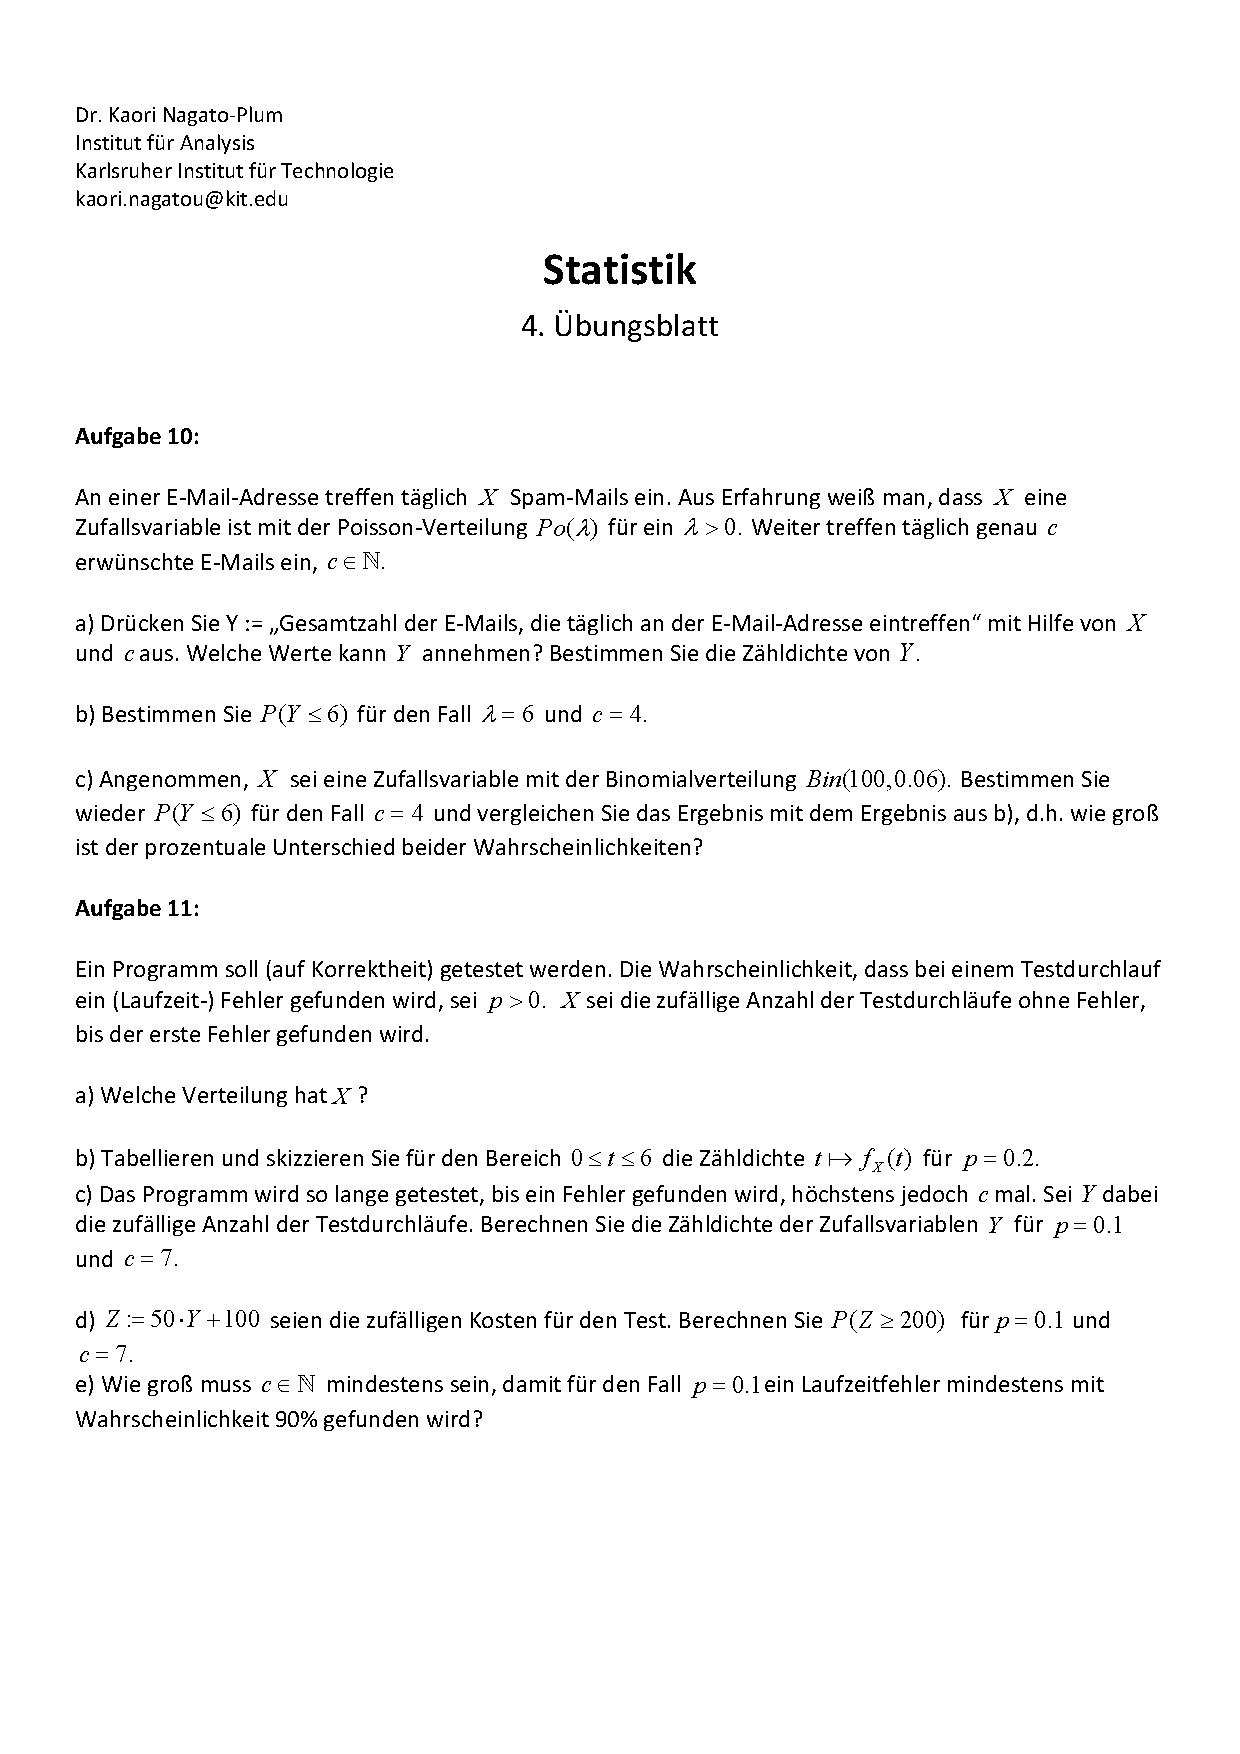
\includegraphics[scale=0.75,page=1]{input/grahix/Aufgabenblatt4.pdf}

Nur AUfgabe 10 war klausurrelevant.

Aufgabe 10 a.\\

Die Zähldichte für $Y$ ist folgend definiert $Y = X+c$. Da $X$ die Werte 0,1... annehmen kann, nimmt $Y$ die Werte c,c+1,c+2,... an. \\

\[f_Y(k)=P(Y=k)=P(X+c=k)=P(X=k-c)\]
\[f_X(k-c)=\begin{cases}e^{\lambda}*\frac{\lambda^{k-c}}{(k-c)!},k\geq c\\
0\end{cases}\]

Aufgabe 10 b.\\

Wegen $Y\geq c =4$ gilt $P(Y\leq 6)=P(Y=4)+P(Y=5)+P(Y=6)$



Die verteilung ist 








\subsection{03.05}

Aufgabe 15 a.\\

Bestimme die Dichtefunktion:

\[F(x)=1-e^{-kx}\]
\[f(x)=k*e^{-kx}\]

Für einen bestimmten Bauteil ist k = 1. Wie groß ist dann die Wahrscheinlichkeit, dass die Lebensdauer 
b. höchstens 1 Jahr \\

\[\Longrightarrow P(L\leq1)=F_1(1)-F_1(0)=1-e^{-1*1}-0=0.6321\]


c. zwischen 1 und 2 Jahren \\

\[ \Longrightarrow P(1 \leq L \leq 2) = F_1(2)-F_1(1) = (1-e^{-1*2}) -0.6321 = 0.2325\]


d. größer als 2 Jahre ist?\\

\[ \Longrightarrow P(L\geq 2) = 1-(F_1(2)-F_1(0))=0.13533\]

\subsection{10.05}

Aufgabe 16 a.\\

\[Y = N (0,16)\]

\[X=\tau + Y\]
\[ Y \sim  N(0,4^2)\]
\[\Longrightarrow X = \tau + Y = (\tau/a) + (1/b) * Y\]
\[\sim  N(\overbrace{a+b\mu}^{=\tau} ,\overbrace{b^2*\sigma ^2}^{= 4^2})\]
\[X \sim N(\tau, 4^2)\]
\[\Longrightarrow P(X\leq 100)\]

b.\\

\[\Phi (\frac{\overbrace{t}^{100}-\overbrace{\mu}^\tau}{\sigma})\]
\[\mu_0 = 1-(P\leq 100) = p_0=\Phi (\frac{\overbrace{t}^{100}-\overbrace{\mu}^{100}}{\sigma})=\Phi(0)=0.5 \]
\[\mu_1 = 1-(P\leq 102) = p_1=\Phi (\frac{\overbrace{t}^{100}-\overbrace{\mu}^{102}}{\sigma})=\Phi(-0.5)= 0.6915\]

c.\\

Jeder der vier Fühler hat die Wahrscheinlichkeit von 50$\%$ anzuschlagen bei der Temperatur 100 Grad es braucht zwei damit der Ventiator angeht.
\[N\sim Bin(4,p)=P(N=k)=\binom{4}{k}*0.5^k*0.5^{4-k}\]
\[P(N=2)+P(N=3)+P(N=4)\]
Die Wahrscheinlichkeit das der Ventilator angeht liegt bei 43.75 Prozent.\\

d.\\

\[p=0.6915\]\[ P(N\geq 1)\]

Aufgabe 17\\
a.\\
\[\mu =2 \vert \sigma =0.5 \vert P(X\leq 3)\]
\[P(N>3) = 1-(X\leq 3)= 1-\Phi _{2,0.5^2}(3)=1-\Phi (\frac{3-2}{0.5} )=\Phi (2)=1-0.97=0.03\]

\subsection{24.05}
Aufgabe 18 ist ein gute Übung für bedingte wahrscheinlichkeit.\\
\textbf{Aufgaben 20a}\\
Als Beispiel für bedingte wahrscheinlichkeit nutzen

Auf einem Mail-Server sind 96\% der ankommenden Mails Spam.\\
a.$)$Die Wahrscheinlichkeit liegt bei 90\% das eine Mail als Spam erkannt wird(d.h. mit 10\% das der Spam durch geht). Die Wahrscheinlichkeit das ein echte Mail als Spam erkannt wird liegt bei 2\%. Welcher Anteil der Mails, sind im langfristigen Mittel Spam-Mails?
\begin{align*}
    S&:= \textrm{der eingehenden Mails sind Spam} &\overline{S}&:= \textrm{nicht Spam}\\
    P&(S)=0.96 &P(\overline{S})&=0.04\\
    P&(S\cap L)= 0.96\cdot 0.90=0.864  &P(S\cap\overline{L})&=0.96\cdot0.10 = 0.096\\
    P&(\overline{S}\cap L)= 0.04\cdot 0.02 = 0.0008 &P(\overline{S}\cap\overline{L})&=0.04\cdot0.98 = 0.0392
\end{align*}
Es kommen 13.52\% der einkommenden Mails durch
\begin{align*}
    P(\overline{L})&= 0.1352\\
    P(S\cap\overline{L})&= 0.096\\
    P(S|\overline{L})&= \frac{P(S\cap \overline{L})}{P(\overline{L})} = \frac{0.096}{0.1352}\approx  0.71
\end{align*}



\end{document}